\documentclass[12pt]{jreport}
\usepackage{comment}
\usepackage{./sty/eclepsf}
\usepackage{tascmac}
\usepackage{tabularx}
\usepackage{listliketab}
\usepackage[longnamesfirst]{natbib}
\usepackage[dvipdfmx]{graphics}
\usepackage[dvipdfmx]{graphicx}
\usepackage[dvipdfmx]{color}
\usepackage{subfigure}
\usepackage{alltt}
\usepackage{here}
\usepackage{afterpage}
\usepackage{./sty/ncodeline}
%\usepackage[dvipdfmx, colorlinks, breaklinks,%
\usepackage[dvipdfmx, breaklinks,%
bookmarks=true, bookmarksnumbered=true,%
bookmarkstype=toc, bookmarksopen=true,bookmarksopenlevel=3,%
pdftitle={RG},%
]{hyperref}
\usepackage{bookmark}

\AtBeginDvi{\special{pdf:tounicode EUC-UCS2}}

\usepackage{fancyhdr}

\usepackage{./sty/doxygenorig}

\usepackage{indentfirst}
\usepackage{url}
\usepackage{listings,./sty/jlisting}

\def\lstlistingname{プログラム}

\lstset{%
 language={C++},
 %backgroundcolor={\color[gray]{.85}},%
 basicstyle={\small\ttfamily},%
 identifierstyle={\small},%
 commentstyle={\small\itshape},%
 keywordstyle={\small\bfseries},%
 ndkeywordstyle={\small\ttfamily},%
 stringstyle={\small\ttfamily},
 frame={tb},
 framesep=1zw,
 breaklines=true,
 numbers=left,%
 xrightmargin=0zw,%
 xleftmargin=1.5zw,%
 numberstyle={\scriptsize},%
 stepnumber=1,
 numbersep=1zw,%
 lineskip=-0.5ex%
}

\usepackage{amssymb}
%\usepackage{supertabular,multirow}

\usepackage{array}
\newcolumntype{M}[1]{>{\centering\arraybackslash}m{#1}}

% A4  size: 297mm*210mm %1pt = 0.35mm
\setlength{\topmargin}{-3.4mm} % 10pt 25.4mm - 3.4mm = 22mm
\setlength{\oddsidemargin}{-0.4mm} % 25.4mm - 0.4mm = 25mm
\setlength{\evensidemargin}{-0.4mm} % 25.4mm - 0.4mm = 25mm
\setlength{\textheight}{231mm} % 660pt % original is 225.75mm 645pt
\setlength{\textwidth}{160mm} % 457pt

\renewcommand{\topfraction}{.99}
\renewcommand{\textfraction}{.0}
\renewcommand{\floatpagefraction}{.99}
\renewcommand{\bibname}{参考文献}


\pagestyle{fancy}
\lhead[]{}

\makeatletter
\def\chaptermark#1{\markboth {\ifnum \c@secnumdepth>\m@ne
\@chapapp\ \thechapter \@chappos\ \fi #1}{}}
\makeatother

% タイトル
\def\title{目的満足度に応じたモビリティ全体制御}
% 英語タイトル
\def\etitle{Mobility for Human Satisfaction}
% 著者(日本語)
\def\author{島津翔太}
% 著者(英語)
\def\eauthor{Shota Shimazu}
% 学部・研究科
\def\dept{慶應義塾大学環境情報学部環境情報学科}
% 学部・研究科(英語)
\def\edept{Keio University Faculity of Environment and Information Studies}

\begin{document}

\pagenumbering{roman}
\begin{titlepage}
  \begin{center}
    \begin{large}
      卒業論文   2019年度(令和1年)\\
      \vspace{24pt}
      \title
      \end{large}
  \end{center}
  \vspace{40em}
  \begin{flushright}
    \large \dept\\
    \author
  \end{flushright}
\end{titlepage}

\thispagestyle{empty}


卒業論文要旨 - 2019年度 (令和1年度)
\begin{center}
\begin{large}
\begin{tabular}{|M{0.97\linewidth}|}
    \hline
      \title \\
    \hline
\end{tabular}
\end{large}
\end{center}

~ \\

\textcolor{red}{修正途中}
自動運転技術の発展により, 我々人間は車を直接コントロールする必要がなくなってきた.
例えば, 車線の自動変更や物体検知による自動ブレーキなどは, 今まで人間が行っていた操作をコンピューターによって行っている.
今後, 自動運転技術はより高度になり, 近い将来人間がハンドルを握らなくともコンピューターによる制御のみで目的地まで到達できるレベルまで発展する可能性がある.
そのような自動運転車が普及した社会において, 自動車各個が個別に行動すると様々な問題が発生する.

第一に, 特定の経路の混雑があげられる.
多数の自動運転車が個別に経路を選択した場合, 特定の道が混雑する問題が発生する.
第二に, 自動運転による使用用途の変化への順応である. 人間による操作が一切行われない完全自動運転が実現する事はすなわち無人運転が可能であることを意味する.
無人運転が可能となった場合, 自動車の保有者が目的地についた後に駐車する必要はなく, 駐車時間中に自動車を使いたい人の元へ迎えに行く無人のヒッチハイクのような行為が可能となる.
このような使用用途の変化に対応するには, 単に目的地までのルートを選択するだけではなく目的地に到達した後の行動も自動運転車が決定する必要がある.

そこで, 本研究では強化学習を用いて自動車の利用者の目的に合わせた経路選択の実験を行った.
実験では, 緊急のミーティングに向かっている, 空腹を感じているなどの利用者の目的や状態などのパターンを予め想定した. そのパターンに対して利用者の目的を達成するルートを選択した場合に強化学習に報酬値を与え, 目的を満たせないルートを選択した場合は罰則値を与える.
これを繰り返すことにより, 強化学習アルゴリズムがより目的を達成するような経路選択を行えるようになると考えられる.

これらの実験を通して, 本研究では正解データなし自律して意思決定を行うアルゴリズムの一種である強化学習を用いたアプローチが人間の目的を満たす意思決定に有効であること. モビリティの経路選択において実用的であることを示す事を示す.

~ \\
キーワード:\\
\underline{1. 機械学習},
\underline{2. 深層強化学習},
\underline{3. モビリティ},
\underline{4. シェアリングエコノミー}
\begin{flushright}
\dept \\
\author
\end{flushright}

\thispagestyle{plain}
\clearpage

Abstract of Bachelor's Thesis - Academic Year 2019
\begin{center}
\begin{large}
\begin{tabular}{|p{0.97\linewidth}|}
    \hline
      \etitle \\
    \hline
\end{tabular}
\end{large}
\end{center}

~ \\
With the development of autonomous driving technology, we humans no longer need to constantly control cars.
For example, automatic lane changes and automatic braking based on object detection are done by computers in the same way that humans have done so far.
In the future, automatic driving technology will become more advanced, and there is a possibility that in the near future, it will be developed to a level where a person can reach a destination only by computer control without grasping the steering wheel.
In a society where such self-driving vehicles are widespread, various problems arise when individual vehicles act individually.

First, there is congestion on specific routes.
If a large number of autonomous vehicles select their own routes individually, there will be a problem of congestion on specific roads.
The second is to adapt to changes in usage by automatic operation. The realization of fully automatic operation without any human intervention means that unmanned operation is possible.
When unmanned driving becomes possible, it is not necessary to park a car after the car owner arrives at the destination, and an act such as an unmanned hitchhiking to pick up a person who wants to use the car during parking time becomes possible.
In order to respond to such changes in usage, it is necessary for the self-driving vehicle not only to select the route to the destination but also to determine the actions to take after reaching the destination.

In this study, therefore, we use reinforcement learning to experiment with route selection according to the purpose of vehicle users.
In the experiment, we assumed the user's purpose and condition such as going to an emergency meeting or feeling hungry. If the user selects a route that achieves the user's purpose for that pattern, we give a reward value to reinforcement learning. If the user selects a route that does not meet the user's purpose, we give a penalty value.
By repeating this process, the reinforcement learning algorithm may be able to select a route that achieves a better goal.

Through these experiments, we hope to show that an approach using reinforcement learning, which is a kind of algorithm that makes independent decisions without correct data, is effective for making decisions that satisfy human objectives and is practical for path selection of mobility.
~ \\
Keywords : \\
\underline{1. Machine Learning},
\underline{2. Reinforcement learning},
\underline{3. Mobility}
\begin{flushright}
\edept \\
\eauthor
\end{flushright}

\thispagestyle{plain}
\clearpage

\tableofcontents\thispagestyle{plain} %目次
\clearpage
\listoffigures\thispagestyle{plain} %図目次
\clearpage
\listoftables\thispagestyle{plain} %表目次
\clearpage

\pagenumbering{arabic}
\chapter{序論}
\label{introduction}

本章では本研究の背景,課題及び手法を提示し,本研究の概要を示す.


\section{背景}
\label{introduction:background}

本章では, 本研究の背景を示す.

\subsection{自動運転}

車における自動運転は1980年代から研究されてきた.
例えば, 欧州で1987年から1995年に行われたEUREKAプロメテウス計画では高速道路における車線の追従や車線の変更などの自動運転の基礎技術が研究された.
現在では, これらの機能は市販の自家用車にも運転をアシストする機能として搭載されている. また, 高速道路など限定した場所であれば人間による介入が不要な一部自動運転が可能となっているものもある.
今後, 将来自動運転技術はより人間による介入を少なくし, 首相官邸ホームページ「官民 ITS 構想・ロードマップ 2017」に定義されたレベル5の完全な自動運転技術も完成する可能性がある.


\subsection{Mobility as a Service}

日本に置いて, 車や鉄道などの交通は高度経済成長期以降, 急速に普及が進み, 旅客・貨物共に主たる移動手段となった. 

しかし, 近年, 交通は単なる移動手段としてだけではなく, 移動や移動に付随する付加価値が求められるようになってきた.

これに対して移動をサービスとして提供しようという試みがあり, Mobility as a Service (通称: MaaS)と呼ばれている.

\subsection{シェアリングエコノミー}

ここは削ると思う
シェアリングエコノミーとは....である. 将来, 人間が介在することのない自動運転が可能になると

\subsection{機械学習}

日本に置いて高度経済成長期以降, 車や鉄道の普及は急速に進み旅客・貨物共に主たる移動手段となった.

しかし, 近年, 交通は単なる移動手段としてだけではなく, 移動や移動に付随する付加価値が求められるようになってきた.
これに対して移動をサービスとして提供しようという試みがあり, Mobility as a Service (通称: MaaS)と呼ばれている.


\subsection{5G}

日本に置いて高度経済成長期以降, 車や鉄道の普及は急速に進み旅客・貨物共に主たる移動手段となった.

しかし, 近年, 交通は単なる移動手段としてだけではなく, 移動や移動に付随する付加価値が求められるようになってきた.
これに対して移動をサービスとして提供しようという試みがあり, Mobility as a Service (通称: MaaS)と呼ばれている.






なお,Bitcoin~\cite{Bitcoin}は関係ない.



\section{本研究の目的}

本研究では, 強化学習を用いたルート選択を試行し人間の満足度を高めるモビリティ制御を目指す.
現状, 自動運転車に代表されるモビリティは個別に行動しており, ルートの選択に置いても人間が与えた目的地への最短経路を選択している.
この場合, 一定時間内に同一方面の目的地を多数設定された場合に特定のルートの混雑が予測される.
本研究では, 



\section{本論文の構成}

本論文における以降の構成は次の通りである.

~\ref{introduction:background}章では,背景を述べる.
~\ref{issue}章では,本研究における問題の定義と,解決するための要件の整理を行う.
~\ref{proposed}章では,本研究の提案手法を述べる.
~\ref{implementation}章では,~\ref{proposed}章で述べたシステムの実装について述べる.
~\ref{evaluation}章では,\ref{issue}章で求められた課題に対しての評価を行い,考察する.
~\ref{conclusion}章では,本研究のまとめと今後の課題についてまとめる.


%%% Local Variables:
%%% mode: japanese-latex
%%% TeX-master: "../thesis"
%%% End:
\chapter{本研究における問題定義と仮説}
\label{issue}

本章では, 第~\ref{background}章で述べた背景から, 現状の自動運転システムが目的としている制御方法の問題点を述べる.

\section{最短経路問題}

%% MARK: あとで背景の章に移動

広く一般的に自動運転車が普及すると, 人間による非合理的なブレーキなどの操作がなくなり渋滞が解消すると言われている.
しかし, 渋滞は車線あたりの交通量に比例し, 一般的に自動車の走行ルートを決定する場合, 現在地から目的地までの最短ルートを選択するため
交通需要の高い経路の交通量は変わらず, 自動運転による渋滞解消の因果関係には疑問が残る.
少なくとも同時間帯に同一地点付近の目的地を設定した車が大量にいた場合に特定のルートが混雑が発生することは避けられないと考えられる.
現状のカーナビゲーションシステムなどに搭載されているような渋滞回避機能であっても, 最短経路の周辺の道路に回避され最短経路を選択するには早いもの順になる状態になる.




\begin{figure}[H]
    \centering  % 図を真ん中に配置
    
\includegraphics[clip,width = 13.0cm]{assets/shorten_route.eps}
    \caption{最短経路問題}  \label{sample}
\end{figure}

  
\section{満足度最適化}

将来のモビリティーのサービス化を進めるにあたり, 目的地までの最短経路の走行では利用者の目的を満たせず満足度を高められない可能性がある.
例えば, 

\section{本研究における問題定義}

現状の強化学習の問題点を列挙し, 整理する.

\subsection{強化学習によるルート選択}

経路選択に強化学習を応用した事例~\cite{DQNRouteSimple}はすでに存在する. 例えば, 下図のような単純な正方形の升目上の任意の座標にスタート地点とゴール地点を設定し, 最短経路を学習するという物である. 
しかし, 実際の道路網は迷路と比較しても非常に複雑であり沿線との接続や経由地などの要素を考慮す

\textcolor{red}{[ここは修正・加筆必要]}
強化学習を応用した場合の精度は未知数である.

\begin{figure}[H]
    \centering  % 図を真ん中に配置
    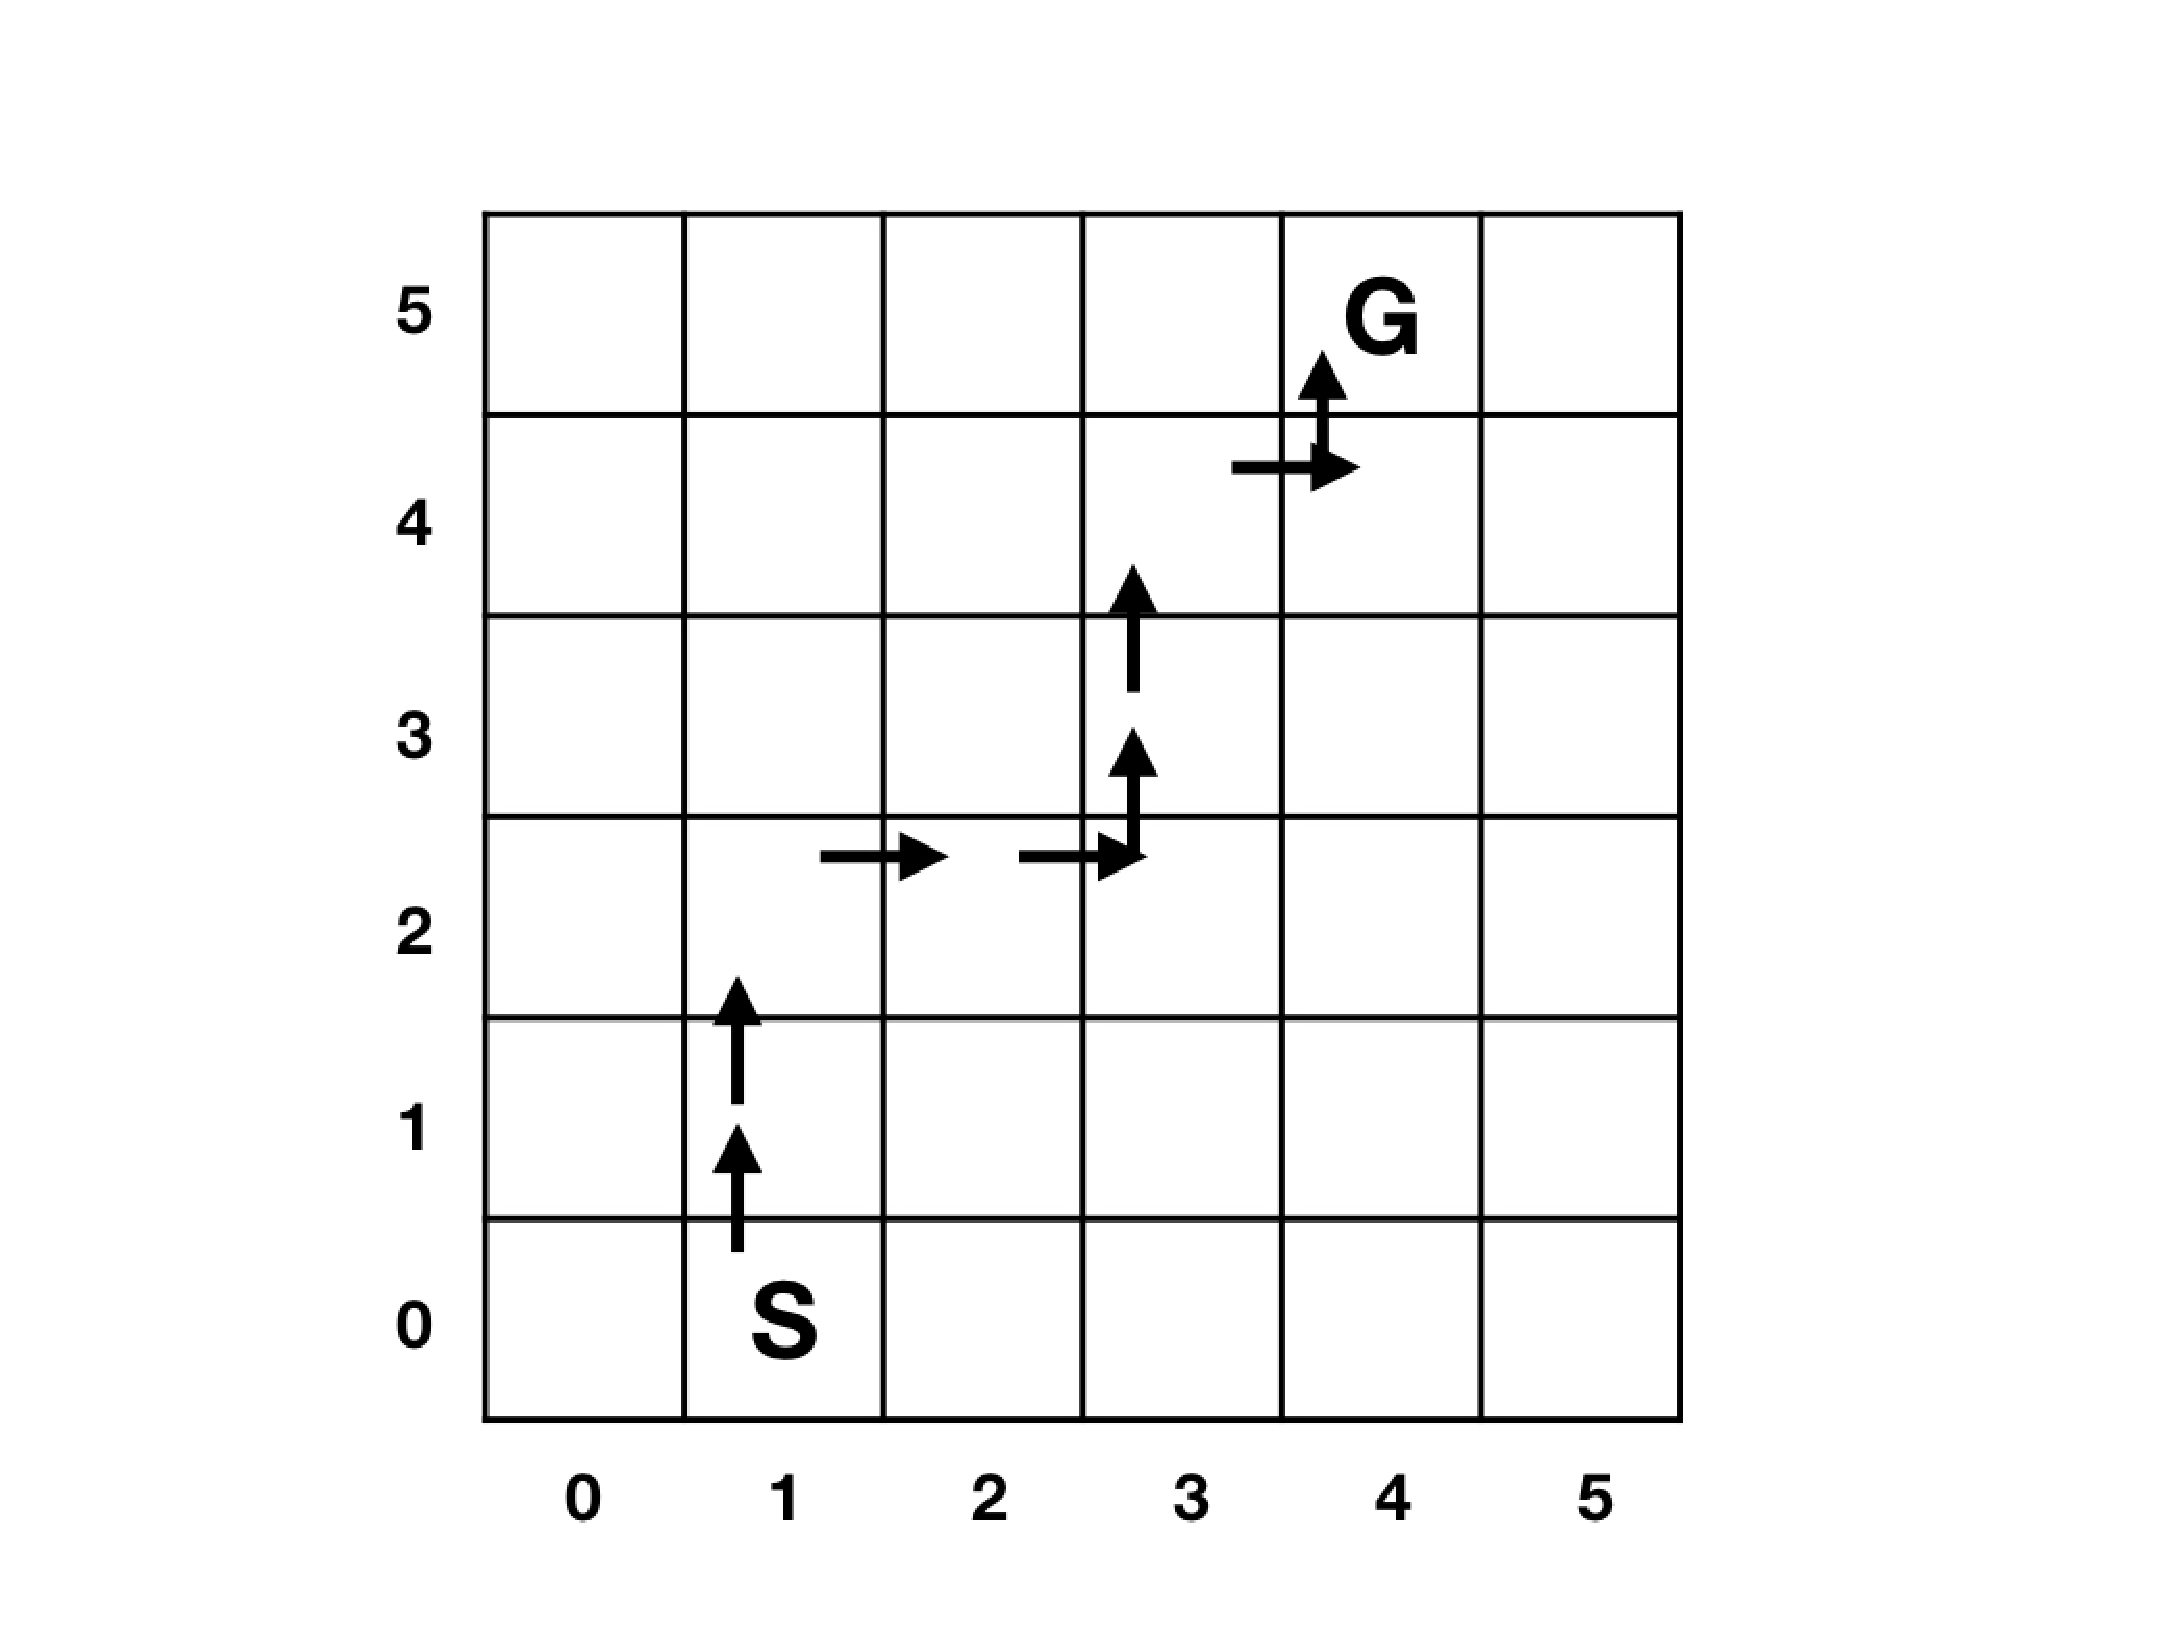
\includegraphics[clip,width = 13.0cm]{assets/rein_simple.eps}
    \caption{強化学習による最短経路検索の結果}  \label{sample}
\end{figure}
  


%% \subsection{ケース策定}   とりあえず仮綴では保留

%% 人間の目的を達成するために  とりあえず仮綴では保留


\section{仮説}

Deep Q Nueral Networkにより学習を繰り返すことで, シミュレーターないでのないでの利用者に最も最適化された経路選択を行うようになると考えた.


%%% Local Variables:
%%% mode: japanese-latex
%%% TeX-master: "./thesis"
%%% End:

\chapter{提案手法}
\label{proposed}

本章では提案手法について述べる.

\section{概要}

本研究では, 人間の状態とモビリティの経路を再現するシミュレータープログラムを開発し実験を行う.
なお, シミュレータープログラムの作成にあたっては以下について仮定を行った.

\begin{itemize}
    \item シミュレーター上での自動車は全てレベル5の完全自動運転ができる物とする
    \item 歩行者や, 自動運転非対応者などは考慮していない
    \item シミュレーターでは予め決められた幹線道路及, 環状線などのバイパス道路のみを考慮し, それ以外の道に関しては考慮しない
    \item 人間の目的を正確に推定するコンピューターシステムもしくはセンサーなどは実在しているものとする. 
\end{itemize}

\subsection{路線網の正規化}

本研究では実際の道路網を参考に仮想の道路網モデルを構築した.
選び出したルートの正則化を行った。実際の地図上にある道路のPOLYLINEデータは道路路線上の点の集合体であり, これを結んだ線分として記録されている. しかし, DQN機械学習モデルでは限られた次元数の行列データしか扱うことができず, そのままではDQNに学習させることができない。
そこで、本研究では、1つのPOLYLINEを交差点毎に分解し交差点に挟まれた1区間を行列の1次元に表し1つの要素とした.
この場合, 区間の距離に関わらず1次元の要素として表すため距離情報が失われる. 従って, ここでは距離を通過難易度dとして環境定義することで距離データを失わないようにした.



\begin{figure}[H]
    \centering  % 図を真ん中に配置
    \includegraphics[clip,width = 13.0cm]{assets/MAP_1.eps}
    \caption{地図上の道路を選択する}  \label{sample}
\end{figure}


\begin{figure}[H]
    \centering  % 図を真ん中に配置
    \includegraphics[clip,width = 13.0cm]{assets/MAP_2.eps}
    \caption{交差点箇所にマークをつける}  \label{sample}
\end{figure}


\begin{figure}[H]
    \centering  % 図を真ん中に配置
    \includegraphics[clip,width = 13.0cm]{assets/MAP_3.eps}
    \caption{地図を省いて路線網だけにした図}  \label{sample}
\end{figure}


\begin{figure}[H]
    \centering  % 図を真ん中に配置
    \includegraphics[clip,width = 13.0cm]{assets/MAP_4.eps}
    \caption{曲線部分を省き直線化する}  \label{sample}
\end{figure}


\begin{figure}[H]
    \centering  % 図を真ん中に配置
    \includegraphics[clip,width = 13.0cm]{assets/MAP_5.eps}
    \caption{区間の長さを等しく正方形にする}  \label{sample}
\end{figure}


\subsection{選択した道路のデータ化}

選択した道路の線形をPostgreSQLにてデータ化を行った. なお, この実験で使用したPostgreSQLには地理情報を扱う拡張であるPostGISをインストールしている.
データ化した内容は, 道路網の一定間隔の座標である. この座標同士を結ぶ線分をPOLYLINE型で記憶し路線名や道路が受け入れることのできる車の第数=Capacityを定義した.

\begin{lstlisting}[caption = 路線データを表すクエリーの例, label = program1]

/*
    テーブル構造の定義
*/
CREATE TABLE geodb_catp_yokohama (
    id                  serial PRIMARY KEY,
    route_name          VARCHAR (100),
    has_spot    VARCHAR (20),
    capacity            INTEGER
);

/*
    線地理情報を記録するPOLYLINE型のカラムを追加
*/
SELECT AddGeometryColumn ('public', 'geodb_catp_yokohama', 'geometry_data', 4326, 'LINESTRING', 2);

/*
    道路の線形を表すデータのレコード
*/
INSERT INTO geodb_catp_yokohama (route_name, has_spot, capacity, geometry_data)
VALUES ('K1',
        'none',
        200,
        ST_GeomFromText('LINESTRING(139.633639 35.445911, 139.632631 35.447126 ...... 139.632323 35.472085)', 4326));
\end{lstlisting}

%%% Local Variables:
%%% mode: japanese-latex
%%% TeX-master: "../bthesis"
%%% End:

\chapter{要素技術}
\label{technical_background}

本章では本研究に用いる手法に関連する要素技術について述べる


\section{機械学習}

機械学習とは広義には, コンピューターが自動的にパターンを学習し人間による明示的な命令がなくとも
特定の課題を自動で実行する技術又はアルゴリズムのことである. 主に, 正解データを与えることによってパターンを学習する教師あり学習,
データのまとまりや相関を求める教師なし学習と繰り返し反復することで価値が最大化するように学習を行う強化学習に分類される.
画像処理や自然言語処理など様々な分野に応用が進んでおり, 画像の検知や自動翻訳など機械学習によって自動化されているものも多い.


\subsection{深層学習}

深層学習とは脳が持つ脳神経系のニューロンをソフトウェアで再現した人工ニューラルネット(ANN)を持つ機械学習アルゴリズムの一つである. 
人間の脳を模したパーセプトロン~\cite{Perceptron}による深層学習自体は1957年から提唱されていた. しかし, 4層以上のパーセプトロンでは過学習や勾配消失問題が発生しやすく計算コストも大きいためあまり普及しなかった.
しかし, 安価なコンピューターでも計算速度が飛躍的に向上したことや勾配消失問題を防止する手法が考案されたことなどから再び注目を集めるようになり, 様々な課題に特価したDNNが考案されている.

例えば, Convolutional Neural Network (CNN)~\cite{CNN}は画像の特徴量抽出に長けており画像認識分野で大きな成果をあげている.
Long short-term memory (LSTM) ~\cite{LSTM}は自動翻訳やテキスト解析など自然言語処理分野で活用されており, 現在では言語だけではなく音楽などにも活用範囲が広がっている.
また, 既存の機械学習の手法に深層学習を組み込んだ事例も散見される.

\subsection{多層パーセプトロン}
パーセプトロンとは


\begin{figure}[H]
    \centering
    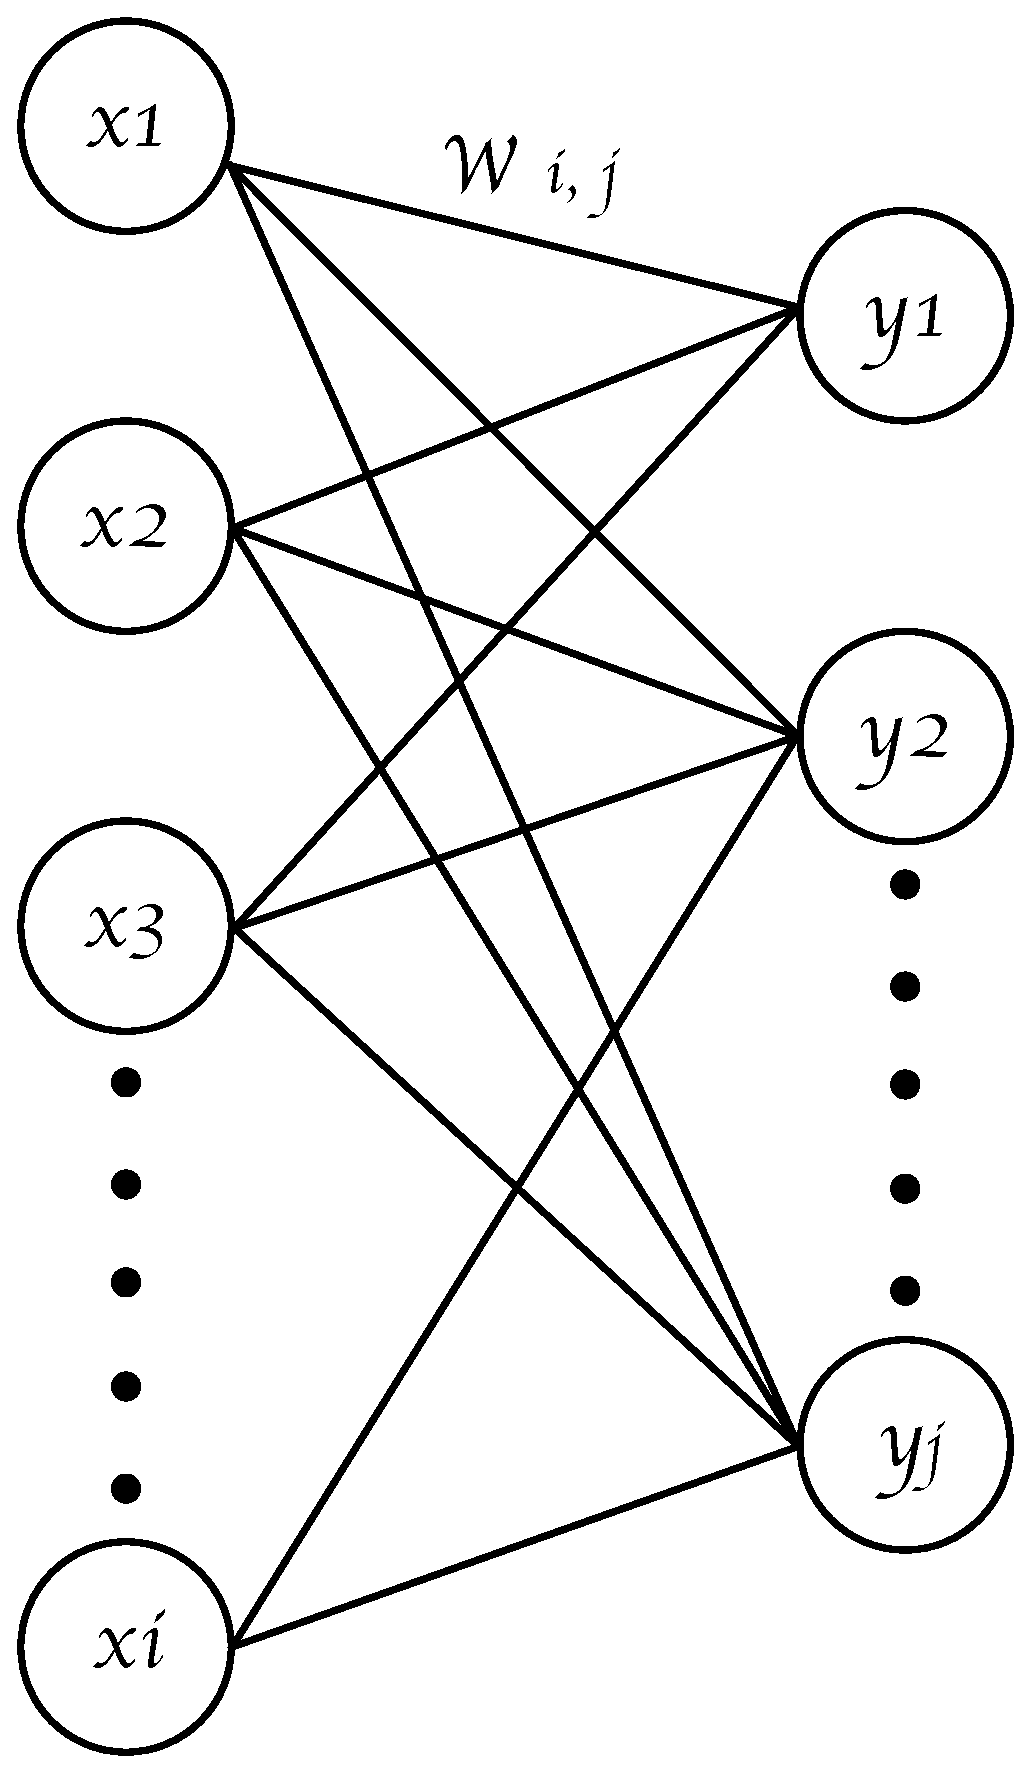
\includegraphics[clip,height = 8.0cm]{assets/perceptron.eps}
    \caption{パーセプトロン}  \label{sample}
\end{figure}

\subsection{強化学習}

強化学習 (Reinforcement learning) ~\cite{ReinforcementLearning}はエージェントと呼ばれる行動主体が現在の状態を観測し価値が最大化する行動を繰り返し選択することにより利益が最大になる行動を学習する機械学習手法の一種である.
強化学習では行動主体であるエージェントと環境を定義する状態と行動した結果による変化, 報酬が定義される.
初期的な強化学習にはマルコフ決定過程~\cite{ReinforcementLearning}やQ学習~\cite{QL}というものがある.

\subsection{深層強化学習}

深層強化学習とは, 強化学習に深層学習を組み合わせた機械学習アルゴリズムである.
強化学習はエージェントとエージェントが動作する環境を定義し, 定義された環境下でエージェントへの報酬が最大化するように学習は行う.

\begin{figure}[H]
    \centering
    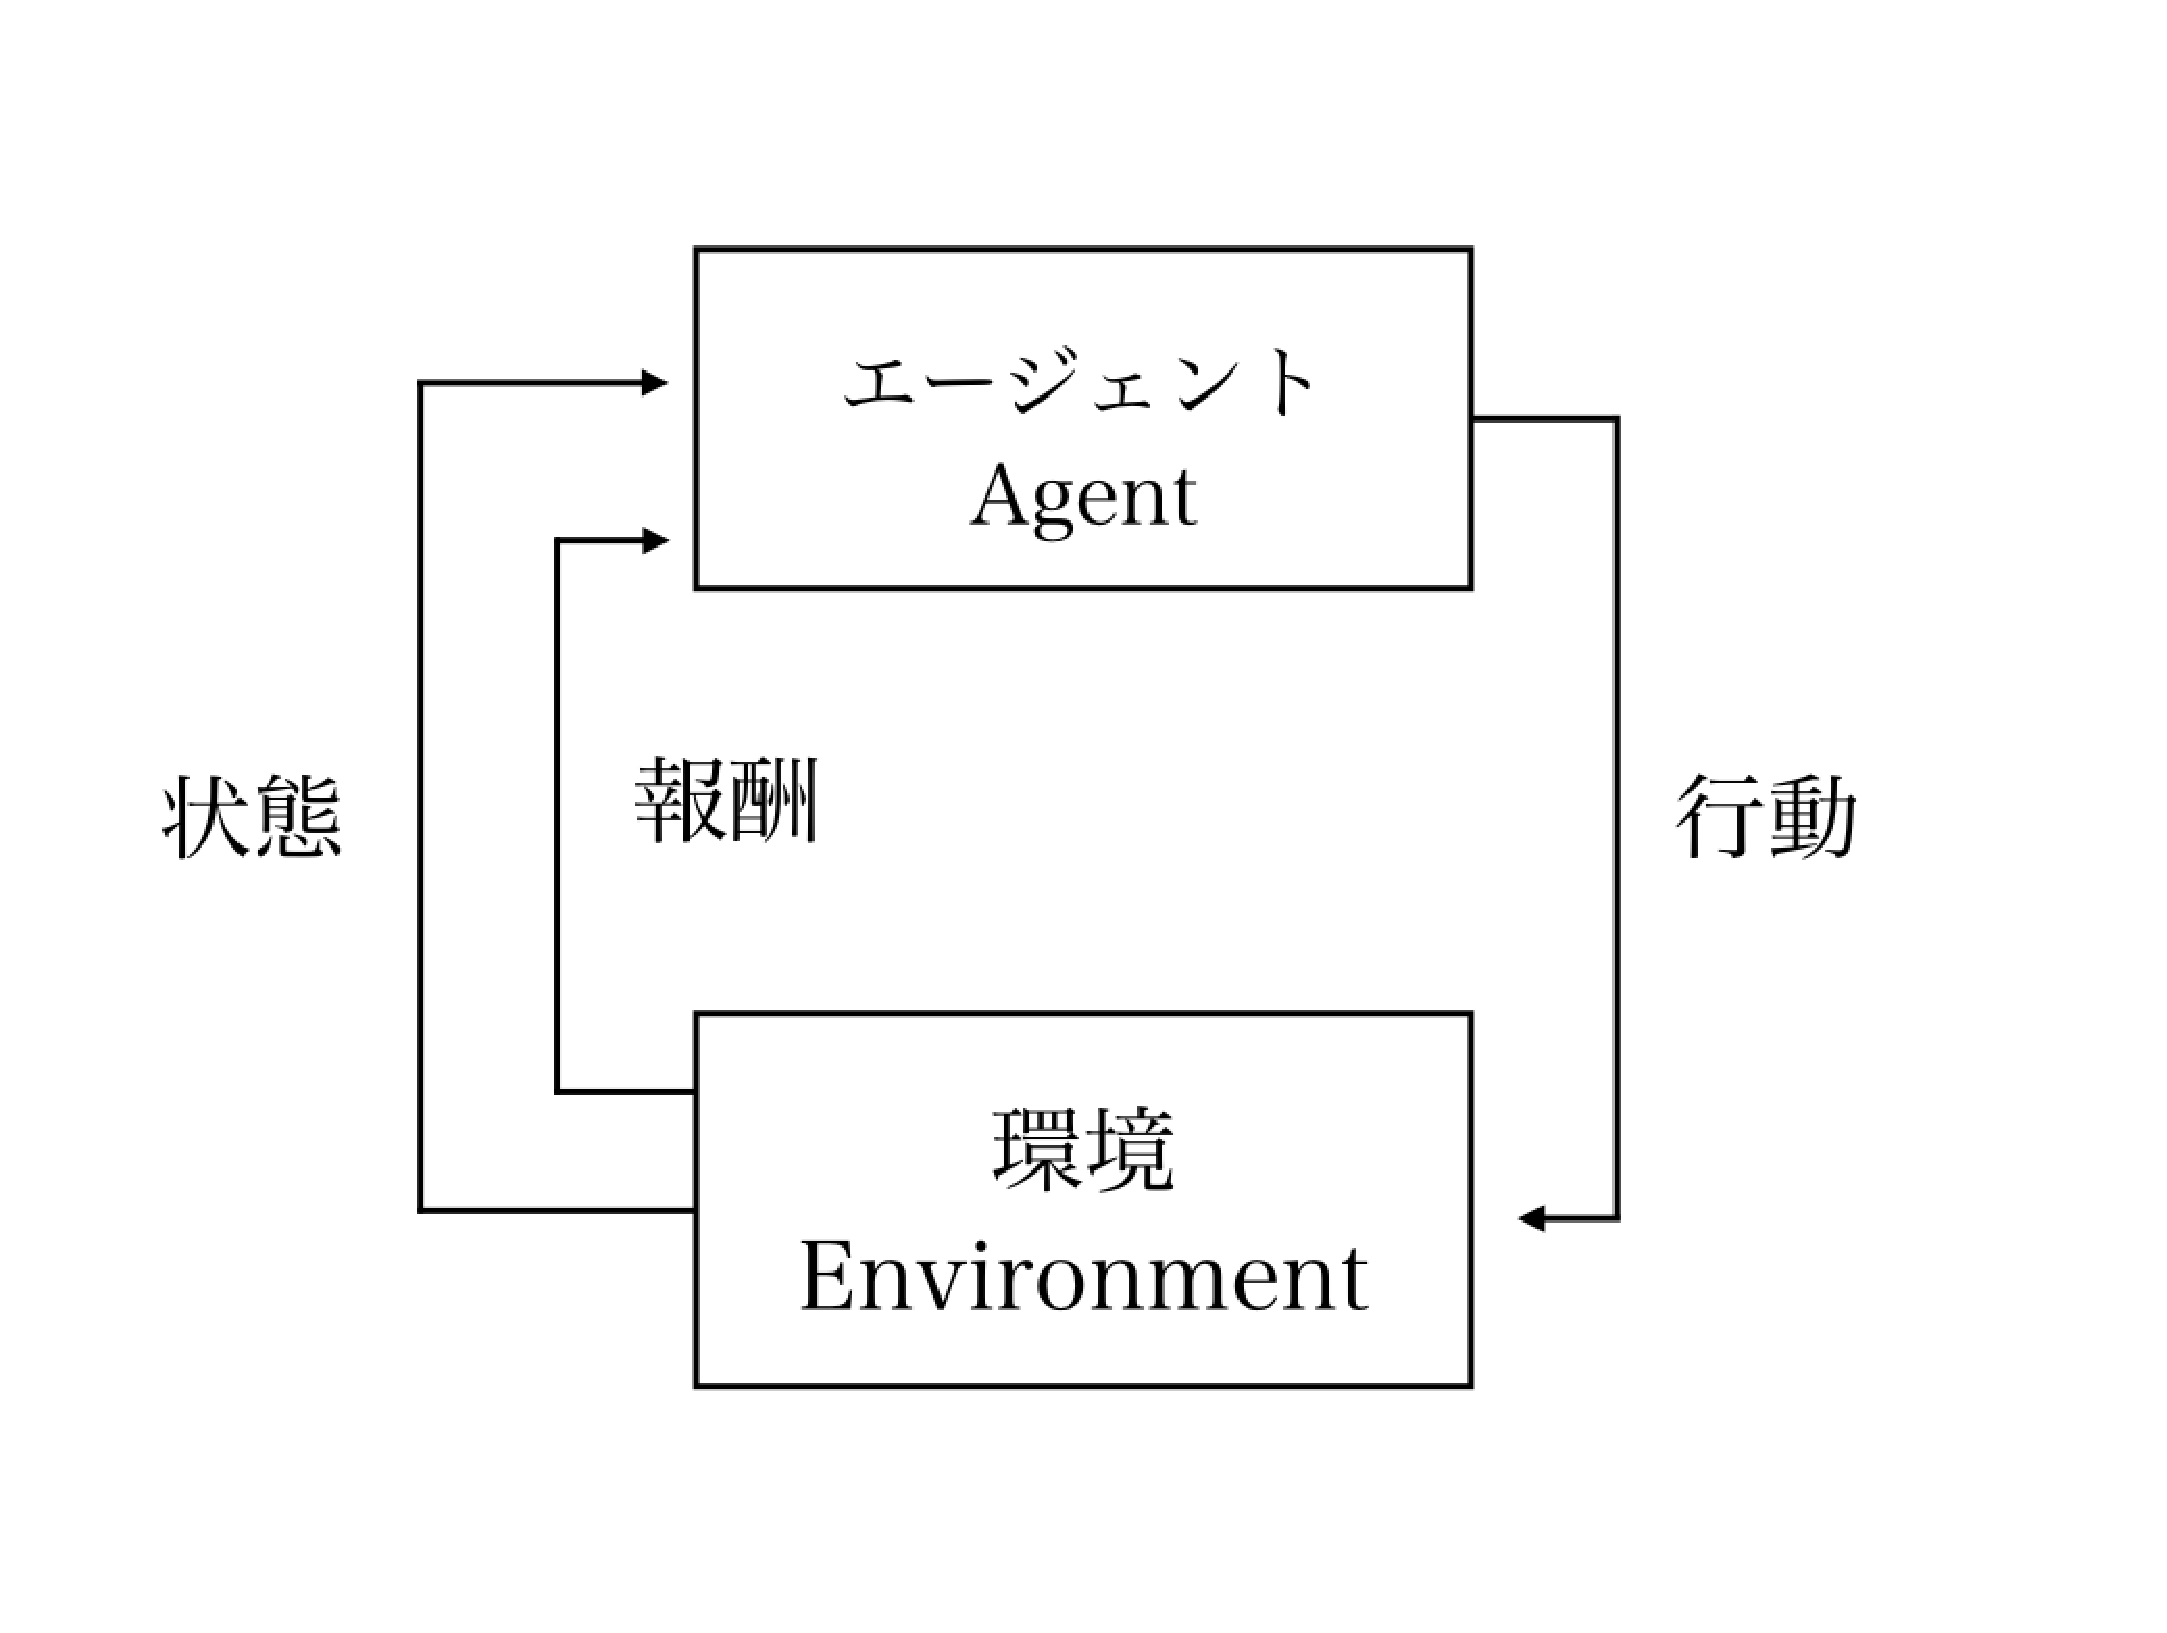
\includegraphics[clip,width = 12.0cm]{assets/reinforcement_learning.eps}
    \caption{強化学習の概念図}  \label{sample}
\end{figure}

\section{Q学習}

Q学習とは初期に考案されたReinforest Learningアルゴリズムの一種であり, 強化学習と呼ばれす.
Q学習による試行は以下のように定義する.

\begin{equation}
    Q(s, a) \approx R(s, a) + \gamma max_{a'} E[Q(s', a')]
\end{equation}

\section{Deep Q Neural Network}

Deep Q Neural Network(DQN~\cite{DQN})はQ学習という強化学習における古典的なアルゴリズムを深層強化学習に応用したものである.
Q学習とは強化学習の一種である. Q学習では実行するルールに対してQ値という値を持たせる.

DQNは深層強化学習とも呼ばれる.


%%% Local Variables:
%%% mode: japanese-latex
%%% TeX-master: "../bthesis"
%%% End:

\chapter{実験}
\label{implementation}

本章では提案手法の実験について述べる.

\section{概要}

本研究では, 以下に述べるコンピュータープログラムを作成し, モビリティや利用者の満足度の変化をコンピューター上で再現する.
作成するプログラムは深層強化学習を行う学習器と環境定義プログラムである.

\section{構成}

この実験での各プログラムやミドルウェアの関係性を~\ref{system_overview}に示す.
pgAdmin~\cite{pgadmin}では, 地図データから選んだ道路の線形データを作成している. その後, 線形データはMap Vectorizerにて正方行列データに変換される.
正方行列に変換された道路データはCNN~\cite{CNN}に入力され, 行動がアウトプットとして出力される. アウトプットされた行動は環境構成プログラムεに入力される.
εはユースケースを定義したクラスと距離表現クラスに定義された内容を基に演算を行い報酬を決定する.

\begin{figure}[H]
  \centering  % 図を真ん中に配置
  \includegraphics[clip,width = 13.0cm]{assets/pgs.eps}
  \caption{システムの関係}  \label{system_overview}
\end{figure}




\begin{table}[h]
  \caption{実験に使用したソフトウェア一覧と役割}
  \label{table:SpeedOfLight}
  \centering
  \begin{tabular}{clll}
    \hline
      名称 & 役割 \\
      \hline \hline
      PostgreSQL~\cite{pgsql} & 道路データの管理 \\
      PostGIS~\cite{postgis} & 地理データの表現と格納 \\
      pgAdmin~\cite{pgadmin} & 地理データのビジュアライズ \\
      QGIS~\cite{qgis} & Open Street Mapの情報読み込み及地理データの閲覧 \\
    \hline
  \end{tabular}
\end{table}


\subsection{仮装道路モデルの作成}

本研究では, 実際の道路を参考にいくつかの道路を抜き出した仮装の道路網を作成した.
選択した道路の線形はPostgreSQL~\cite{pgsql}にてデータ化を行った. なお, この実験で使用したPostgreSQL~\cite{pgsql}には地理情報を扱う拡張であるPostGIS~\cite{postgis}をインストールしている.
データ化した内容は, 道路網の一定間隔の座標である. この座標同士を結ぶ線分をPOLYLINE型で記憶し路線名や道路が受け入れることのできる車の台数をCapacityとして定義した.


\begin{figure}[H]
  \centering  % 図を真ん中に配置
  \includegraphics[clip,width = 13.0cm]{assets/scn1.eps}
  \caption{pgadminにて道路データを地上に可視化した画面}  \label{system_overview}
\end{figure}



\begin{lstlisting}[caption = 路線データを表すクエリーの例, label = program1]

/*
    テーブル構造の定義
*/
CREATE TABLE geodb_catp_yokohama (
    id                  serial PRIMARY KEY,
    route_name          VARCHAR (100),
    has_spot    VARCHAR (20),
    capacity            INTEGER
);

/*
    線地理情報を記録するPOLYLINE型のカラムを追加
*/
SELECT AddGeometryColumn ('public', 'geodb_catp_yokohama', 'geometry_data', 4326, 'LINESTRING', 2);

/*
    道路の線形を表すデータのレコード
*/
INSERT INTO geodb_catp_yokohama (route_name, has_spot, capacity, geometry_data)
VALUES ('K1',
        'none',
        200,
        ST_GeomFromText('LINESTRING(139.633639 35.445911, 139.632631 35.447126 ...... 139.632323 35.472085)', 4326));
\end{lstlisting}



\section{Deep Q Neural Network Model}

この実験ではDeep Q Nueral Networkによる強化学習を行う学習器を構築するプログラムをPython言語を用いて作成した.
このプログラムは深層強化学習を形成するニューラルネットワークを定義したプログラムである.
ライブラリとしてTensorFlow及びKerasを用いた.


\begin{lstlisting}[caption = DQNの深層学習部分を形成するモデル, label = program1]
  from tensorflow.keras.models import Sequential
  from tensorflow.keras.layers import (
    Dense,
    Activation,
    Flatten,
    Convolution2D,
    Permute
  )
  from tensorflow.keras.optimizers import Adam
  import tensorflow.keras.backend as K
  
  
  def dqnmodel():
      model = Sequential()
  
      model.add(Permute((17, 17, 1), input_shape=input_shape))
  
      model.add(Convolution2D(32, (8, 8), strides=(4, 4)))
      model.add(Activation('relu'))
      model.add(Convolution2D(64, (4, 4), strides=(2, 2)))
      model.add(Activation('relu'))
      model.add(Convolution2D(64, (3, 3), strides=(1, 1)))
      model.add(Activation('relu'))
      model.add(Flatten())
      model.add(Dense(512))
      model.add(Activation('relu'))
      model.add(Dense(nb_actions))
      model.add(Activation('linear'))
  
      return model  
\end{lstlisting}
  
  

\section{Map Vectorizer}

Data SerializerはPostgreSQLサーバー上に記録された経路などの地理データーを上述したDeep Q Neural Network
に学習させるためのデーター変換を行うプログラムである.
開発言語はPythonである. PostgreSQLから受け取った道路のPOLYLINEデータから各座標点を抽出し, 座上間を繋いだ



\begin{figure}[H]
  \centering  % 図を真ん中に配置
  \includegraphics[clip,width = 13.0cm]{assets/map2vector.eps}
  \caption{地理データをDQNが学習可能な正方行列データに変換する}  \label{map2vector}
\end{figure}



\section{学習用コンテナの作成}

Docker\footnote{DockerはOS仮想化システムの一種である. VirtualBoxなどの完全仮想化
ソフトウェアとは異なり、ゲストOSの命令セットをホストOSのカーネルの命令セットにコンバートすることにより仮想化を実現している.
これにより, ハードウェアの仮想化を伴わないためオーバーヘッドが少なく機械学習のような計算量の多い課題に適していると言える.}
本研究では, 機械学習システムの実行環境として採用をした.
-----
主に, Pythonの実行環境系やライブラリなどをUbuntu18.04ベースのコンテナを作成した.
このコンテナには本研究で用いた機械学習システムが依存するTensorFlowの実行環境が用意されている.

\section{本研究で用いる環境定義アルゴリズム}

ここにアルゴリズムを示す

\textbf{for} Routelist

\ \ \ \ 評価関数

\textbf{end for}


\section{環境定義クラス}

\begin{lstlisting}[caption = 環境を構築するクラス, label = program1]

class CATPEnvironment:

  def __init__(self, evaluator, step_t):
      self._evaluator = evaluator
      self._step = step_t
      self._rewords = [ ]

  # Register or memory agent action flow.
  def act(self, act_obj):
      res = act_obj.run()
      rewords = self._evaluator(res)

      self._rewords.append(rewords)
  
  # Calculate environment diff and save environment.
  def commit(self):
      return sum(self._rewords)
  
  # Clear all environment to initial.
  def reset(self):
      total_reword = sum(self._rewords)

  def _capacity_validate(self, route_id):
      if True:
          return -10
\end{lstlisting}
  




\begin{lstlisting}[caption = 行動を定義するクラス, label = program1]

class CATPAction:

  def __init__(self):
    pass

  def reset(self):
    print("Reset environment")

  # Register agent action to environment
  def act(self, act_obj):
    pass

  # Calculate environment diff
  def commit(self):
    print("Committing environment...")

  def _capacity_validate(self, route_id):  
    if True:
        return -10  
\end{lstlisting}
  


%%% Local Variables:
%%% mode: japanese-latex
%%% TeX-master: "../bthesis"
%%% End:

\chapter{評価}
\label{evaluation}

本章では,提案システムの評価について述べる.


\section{評価内容}

ああああああ

%%% Local Variables:
%%% mode: japanese-latex
%%% TeX-master: "./thesis"
%%% End:

\chapter{結論}
\label{conclusion}

本章では,本研究のまとめと今後の課題を示す.

\section{本研究のまとめ}

実験が全て完了したのちにまとめる

\section{本研究の課題}

本研究では, 自動車に限りモビリティーの利用者の満足度を高める経路制御を行う機械的な手法に取り組んだ.
しかし,

\subsection{想定環境の貧弱さ}

本研究では, 事前に選び出した幹線道路とその周辺にある主たる施設のみの仮想環境をソフトウェアで再現した. 
しかし, 実際には交通機関は自動車意外にもあり鉄道やバスなどの大量輸送型の交通機関

\subsection{学習器の連携}

本研究では深層強化学習が利用者の満足度を高めるという視点で制御を行えるか実験を行った. ただ, 実際に本研究

%%% Local Variables:
%%% mode: japanese-latex
%%% TeX-master: "../thesis"
%%% End:

\appendix
\chapter{APPENDIX}


\section{本研究の実験に用いたDocker環境にインストールしたPythonパッケージ}

下記はpip freeze\footnote{pipはPythonのライブラリなどをインストールするパッケージマネージャー}コマンドの実行結果である. 本研究の実験に使用したDockerコンテナ上のOSには以下のPythonパッケージを用いている.

\begin{lstlisting}[caption = pip freezeコマンドの実行結果, label = program1]
absl-py==0.9.0
asn1crypto==0.24.0
astor==0.8.1
attrs==19.3.0
backcall==0.1.0
bleach==3.1.0
cachetools==4.0.0
certifi==2019.11.28
chardet==3.0.4
cloudpickle==1.2.2
cryptography==2.1.4
cycler==0.10.0
decorator==4.4.1
defusedxml==0.6.0
entrypoints==0.3
enum34==1.1.6
future==0.18.2
gast==0.2.2
google-auth==1.10.0
google-auth-oauthlib==0.4.1
google-pasta==0.1.8
grpcio==1.26.0
gym==0.15.4
h5py==2.10.0
idna==2.6
imageio==2.6.1
importlib-metadata==1.4.0
ipykernel==5.1.3
ipython==7.11.1
ipython-genutils==0.2.0
ipywidgets==7.5.1
jedi==0.15.2
Jinja2==2.10.3
jsonschema==3.2.0
jupyter==1.0.0
jupyter-client==5.3.4
jupyter-console==6.0.0
    jupyter-core==4.6.1
    jupyter-http-over-ws==0.0.7
    Keras==2.3.1
    Keras-Applications==1.0.8
    Keras-Preprocessing==1.1.0
    keras-rl2==1.0.3
    keyring==10.6.0
    keyrings.alt==3.0
    kiwisolver==1.1.0
    Markdown==3.1.1
    MarkupSafe==1.1.1
    matplotlib==3.1.2
    mistune==0.8.4
    more-itertools==8.0.2
    nbconvert==5.6.1
    nbformat==5.0.3
    networkx==2.4
    notebook==6.0.2
    numpy==1.18.1
    oauthlib==3.1.0
    opencv-python==4.1.2.30
    opt-einsum==3.1.0
    pandocfilters==1.4.2
    parso==0.5.2
    pexpect==4.7.0
    pickleshare==0.7.5
    Pillow==7.0.0
    prometheus-client==0.7.1
    prompt-toolkit==2.0.10
    protobuf==3.11.2
    ptyprocess==0.6.0
    pyasn1==0.4.8
    pyasn1-modules==0.2.8
    pycrypto==2.6.1
    pyglet==1.3.2
    Pygments==2.5.2
    pygobject==3.26.1
    pyparsing==2.4.6
    pyrsistent==0.15.7
    python-dateutil==2.8.1
    PyWavelets==1.1.1
    pyxdg==0.25
    PyYAML==5.3
    pyzmq==18.1.1
    qtconsole==4.6.0
    requests==2.22.0
    requests-oauthlib==1.3.0
    rsa==4.0
    scikit-image==0.16.2
    scipy==1.4.1
    SecretStorage==2.3.1
    Send2Trash==1.5.0
    six==1.13.0
    tb-nightly==1.14.0a20190603
    tensorboard==2.1.0
    tensorflow==2.0.0b1
    tensorflow-estimator==2.1.0
    termcolor==1.1.0
    terminado==0.8.3
    testpath==0.4.4
    tf-estimator-nightly==1.14.0.dev2019060501
    tornado==6.0.3
    traitlets==4.3.3
    urllib3==1.25.7
    wcwidth==0.1.8
    webencodings==0.5.1
    Werkzeug==0.16.0
    widgetsnbextension==3.5.1
    wrapt==1.11.2
    zipp==0.6.0
\end{lstlisting}
    
    

\section{実験を行ったDockerコンテナの定義ファイル}

本研究では以下の定義ファイルを使用してDocker実験用環境\footnote{docker-compose upコマンドによりDockerfile, docker-compose.yml両定義ファイルに従ったコンテナが作成される}を構築した.

\begin{lstlisting}[caption = Dockerfileの定義, label = program1]
FROM tensorflow/tensorflow:latest-py3-jupyter
LABEL maintainer="shotastage"
RUN apt-get update -y
RUN apt-get install libsm6 libxrender1 libxext6 python-opengl -y
RUN pip install --upgrade pip
RUN pip install -q keras scikit-image keras-rl2 gym
RUN mkdir /catp/
RUN chmod 777 /catp/
\end{lstlisting}



\begin{lstlisting}[caption = docker-compose.ymlの定義, label = program1]
version: '3.7'
services:
    tensorflow:
        build:
            context: .
            dockerfile: Dockerfile
        container_name: tensorflow
        volumes:
            - ./dqncatp:/catp/dqncatp/
            - ./catpvalidator:/catp/catpvalidator/
            - ./catptools:/catp/catptools/
            - ./catpframework:/catp/catpframework/
        tty: true
        command: /bin/bash
        ports:
            - 8889:8889
    
\end{lstlisting}
    


\chapter*{謝辞}
\addcontentsline{toc}{chapter}{謝辞}
\label{thanks}

本論文の執筆にあたり,ご指導頂いた慶應義塾大学環境情報学部村井純博士,同学部教
授中村修博士,同学部教授楠本博之博士,同学部准教授高汐一紀博士,同学部教授三次仁
博士,同学部准教授植原啓介博士,同学部准教授中澤仁博士,同学部準教授 Rodney D.
Van Meter III 博士,同学部教授武田圭史博士,同大学政策・メディア研究科特任准教授
鈴木茂哉博士,同大学政策・メディア研究科特任准教授佐藤 雅明博士,同大学 SFC 研究
所上席所員斉藤賢爾博士に感謝致します.

特に斉藤氏には重ねて感謝致します.研究活動の中で様々な視点での助言をいただきました.




%%% Local Variables:
%%% mode: japanese-latex
%%% TeX-master: "../yummy_bthesis"
%%% End:


\renewcommand{\thechapter}{\Alph{chapter}}
\setcounter{chapter}{0}
\vspace{-5mm}


\bibliographystyle{unsrt}\pagestyle{plain}
\bibliography{./bib/cites}\pagestyle{plain}
\thispagestyle{plain}%bibtex


\end{document}

%%% Local Variables:
%%% mode: japanese-latex
%%% TeX-master: t
%%% End:
